\documentclass[12pt, a4paper]{article}
\usepackage{amsmath}
\usepackage{amssymb}
\usepackage{geometry}
\usepackage{graphicx}
\usepackage[american, siunitx]{circuitikz}
\usepackage{pgfplots}
\pgfplotsset{compat=1.18}
\usetikzlibrary{calc}
\usepackage[colorlinks=true, allcolors=black]{hyperref}

% Document Formatting
\geometry{a4paper, margin=1in}
\linespread{1.2}

\title{\textbf{New Capacitor Problems \& Solutions}}
\author{}
\date{\today}

\begin{document}
\maketitle

\section*{New Problems: Capacitors}

Here are three new problems designed to test the same core concepts of capacitor networks, dielectrics, and AC circuits, complete with detailed explanations and solutions.

\subsection{Problem 1: The Alternative Infinite Ladder}
\noindent\textbf{Question:} An infinite capacitor ladder, constructed with capacitors of $C = \SI{2.0}{\micro\farad}$, is connected to a \SI{100}{\volt}, \SI{60}{\hertz} AC power supply. What is the RMS current drawn from the supply?

\begin{figure}[htbp]
\centering
\begin{circuitikz}[scale=1]
    \draw (0,0) to[sV, l=\SI{100}{V} \SI{60}{Hz}] (0,2.5)
          to[ammeter] (1.5,2.5)
          to[C, l=$C$] (3.5,2.5);
    \draw (3.5,2.5) -- (3.5,1.5) to[C, l=$C$, mirror] (3.5,0);
    \draw (3.5,2.5) to[C, l=$C$] (5.5,2.5);
    \draw (5.5,2.5) -- (5.5,1.5) to[C, l=$C$, mirror] (5.5,0);
    \draw (5.5,2.5) to[C, l=$C$] (7.5,2.5);
    \draw (7.5,2.5) -- (7.5,1.5) to[C, l=$C$, mirror] (7.5,0);
    \draw (0,0) -- (7.5,0);
    \draw[dashed, thick, ->] (7.5,2.5) -- (8.5,2.5);
    \draw[dashed, thick, ->] (7.5,0) -- (8.5,0);
    \node[align=center] at (8.5,1.25) {Repeat to \\ infinity...};
\end{circuitikz}
\caption{The infinite L-C ladder network.}
\end{figure}

\subsubsection*{Explanation \& Solution}
\begin{enumerate}
    \item \textbf{Set up the Self-Similarity Equation:}
    Let the equivalent capacitance be $C_{eq}$. The circuit is equivalent to one capacitor $C$ in series with the parallel combination of another capacitor $C$ and the rest of the ladder ($C_{eq}$).
    $$ C_{eq} = \left( \frac{1}{C} + \frac{1}{C + C_{eq}} \right)^{-1} $$
    $$ \frac{1}{C_{eq}} = \frac{1}{C} + \frac{1}{C + C_{eq}} $$
    
    \item \textbf{Solve for $C_{eq}$:}
    Rearrange into a quadratic equation:
    $$ \frac{1}{C_{eq}} = \frac{(C + C_{eq}) + C}{C(C + C_{eq})} $$
    $$ C(C + C_{eq}) = C_{eq}(2C + C_{eq}) $$
    $$ C^2 + C C_{eq} = 2C C_{eq} + C_{eq}^2 $$
    $$ C_{eq}^2 + C C_{eq} - C^2 = 0 $$
    Using the quadratic formula, and taking the positive root for capacitance:
    $$ C_{eq} = \frac{-C + \sqrt{C^2 - 4(1)(-C^2)}}{2} = C \left( \frac{\sqrt{5}-1}{2} \right) $$
    Given $C = \SI{2.0}{\micro\farad}$:
    $$ C_{eq} = (\SI{2.0e-6}{\farad}) \left( \frac{2.236 - 1}{2} \right) \approx \SI{1.236e-6}{\farad} $$

    \item \textbf{Calculate Capacitive Reactance ($X_C$):}
    $$ X_C = \frac{1}{2\pi f C_{eq}} = \frac{1}{2\pi (\SI{60}{\hertz})(\SI{1.236e-6}{\farad})} \approx \SI{2146}{\ohm} $$

    \item \textbf{Calculate the RMS Current ($I_{rms}$):}
    $$ I_{rms} = \frac{V_{rms}}{X_C} = \frac{\SI{100}{\volt}}{\SI{2146}{\ohm}} \approx \SI{0.0466}{\ampere} $$
\end{enumerate}
\textbf{Answer:} The RMS current drawn from the supply is \textbf{\SI{46.6}{mA}}.

\newpage

\subsection{Problem 2: Dielectric Insertion (Constant Charge)}
\noindent\textbf{Question:} A parallel plate capacitor with capacitance $C = \SI{10}{\micro\farad}$ is charged by a \SI{12}{\volt} battery. The battery is then disconnected. Afterwards, a dielectric slab with a dielectric constant $\kappa = 4.0$ is inserted, completely filling the space between the plates. What is the final voltage across the capacitor and the final energy stored?

\begin{figure}[htbp]
\centering
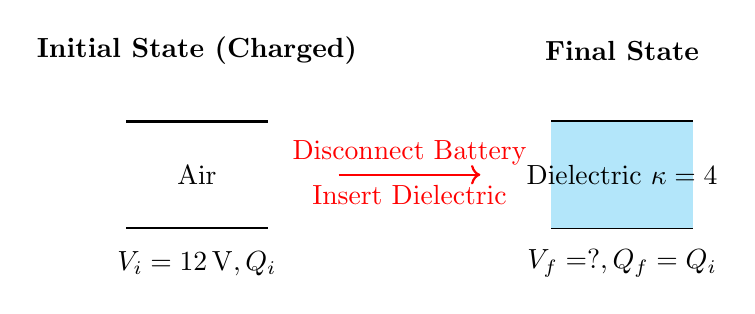
\begin{tikzpicture}[scale=0.9]
    % Initial State
    \node at (0, 2.5) {\textbf{Initial State (Charged)}};
    \draw[thick] (-1,0) -- (1,0);
    \draw[thick] (-1,1.5) -- (1,1.5);
    \node at (0, 0.75) {Air};
    \node at (0, -0.5) {$V_i = \SI{12}{\volt}, Q_i$};
    \draw[->, thick, red] (2, 0.75) -- (4, 0.75) node[midway, above] {Disconnect Battery} node[midway, below] {Insert Dielectric};

    % Final State
    \node at (6, 2.5) {\textbf{Final State}};
    \draw[thick] (5,0) -- (7,0);
    \draw[thick] (5,1.5) -- (7,1.5);
    \fill[cyan!30] (5,0) rectangle (7,1.5);
    \node at (6, 0.75) {Dielectric $\kappa=4$};
    \node at (6, -0.5) {$V_f = ?, Q_f = Q_i$};
\end{tikzpicture}
\caption{Process of inserting a dielectric with the battery disconnected.}
\end{figure}

\subsubsection*{Explanation \& Solution}
\begin{enumerate}
    \item \textbf{Calculate the Initial Charge ($Q$):}
    When connected to the battery, the capacitor stores a charge $Q$. After disconnection, this charge is trapped and remains constant.
    $$ Q = C_i V_i = (\SI{10e-6}{\farad})(\SI{12}{\volt}) = \SI{120e-6}{\coulomb} = \SI{120}{\micro\coulomb} $$

    \item \textbf{Calculate the Final Capacitance ($C_f$):}
    Inserting the dielectric increases the capacitance by a factor of $\kappa$.
    $$ C_f = \kappa C_i = (4.0)(\SI{10}{\micro\farad}) = \SI{40}{\micro\farad} $$

    \item \textbf{Calculate the Final Voltage ($V_f$):}
    Since charge $Q$ is constant, the voltage must decrease.
    $$ V_f = \frac{Q}{C_f} = \frac{\SI{120e-6}{\coulomb}}{\SI{40e-6}{\farad}} = \SI{3.0}{\volt} $$

    \item \textbf{Calculate the Final Stored Energy ($U_f$):}
    The energy stored is given by $U = \frac{1}{2}QV$.
    $$ U_f = \frac{1}{2} Q V_f = \frac{1}{2} (\SI{120e-6}{\coulomb})(\SI{3.0}{\volt}) = \SI{1.8e-4}{\joule} $$
\end{enumerate}
\textbf{Answer:} The final voltage is \textbf{\SI{3.0}{V}} and the final stored energy is \textbf{\SI{180}{\micro\joule}}.

\newpage

\subsection{Problem 3: Complex Dielectric Stacking}
\noindent\textbf{Question:} A parallel plate capacitor has plate area $A$ and separation $d$. The space between the plates is filled with three dielectrics as shown. The top half is filled with a material of dielectric constant $\kappa_1$. The bottom half is split into two equal sections, filled with materials of dielectric constants $\kappa_2$ and $\kappa_3$. Find the equivalent capacitance.

\begin{figure}[htbp]
\centering
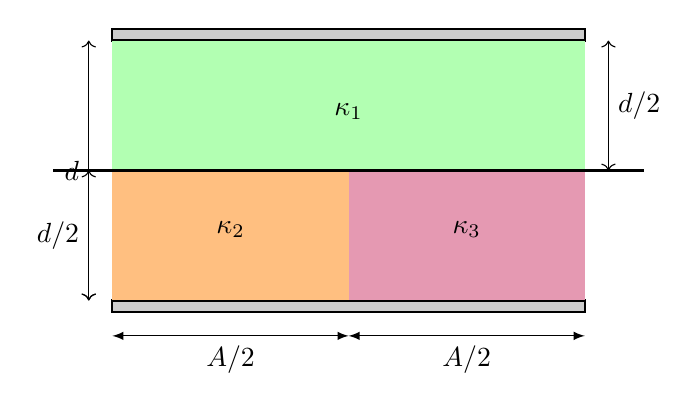
\begin{tikzpicture}[scale=1.5]
    % Plates
    \draw[fill=gray!40, thick] (-2,-1.1) rectangle (2,-1.2);
    \draw[fill=gray!40, thick] (-2,1.1) rectangle (2,1.2);

    % Dielectrics
    \fill[green!30] (-2,0) rectangle (2,1.1);
    \fill[orange!50] (-2,-1.1) rectangle (0,0);
    \fill[purple!40] (0,-1.1) rectangle (2,0);

    % Labels
    \node at (0,0.5) {$\kappa_1$};
    \node at (-1,-0.5) {$\kappa_2$};
    \node at (1,-0.5) {$\kappa_3$};

    % Dimensions
    \draw[<->] (-2.2, -1.1) -- (-2.2, 1.1) node[midway, left] {$d$};
    \draw[<->] (2.2, 0) -- (2.2, 1.1) node[midway, right] {$d/2$};
    \draw[<->] (-2.2, -1.1) -- (-2.2, 0) node[midway, left] {$d/2$};
    \draw[<->, >=latex] (-2, -1.4) -- (0, -1.4) node[midway, below] {$A/2$};
    \draw[<->, >=latex] (0, -1.4) -- (2, -1.4) node[midway, below] {$A/2$};
    \draw[thick] (-2.5,0) -- (2.5,0);
\end{tikzpicture}
\caption{Capacitor with three dielectrics in a different configuration.}
\end{figure}

\subsubsection*{Explanation \& Solution}
\begin{enumerate}
    \item \textbf{Deconstruct the Capacitor:}
    Model this as three capacitors: $C_1$ (top half), $C_2$ (bottom-left), and $C_3$ (bottom-right). $C_2$ and $C_3$ are in parallel, and this combination ($C_{23}$) is in series with $C_1$.

    \item \textbf{Calculate Individual Capacitances:}
    Let the base capacitance be $C_0 = \frac{\epsilon_0 A}{d}$.
    \begin{align*}
        C_1 &= \kappa_1 \frac{\epsilon_0 A}{d/2} = 2\kappa_1 \frac{\epsilon_0 A}{d} = 2\kappa_1 C_0 \\
        C_2 &= \kappa_2 \frac{\epsilon_0 (A/2)}{d/2} = \kappa_2 \frac{\epsilon_0 A}{d} = \kappa_2 C_0 \\
        C_3 &= \kappa_3 \frac{\epsilon_0 (A/2)}{d/2} = \kappa_3 \frac{\epsilon_0 A}{d} = \kappa_3 C_0
    \end{align*}

    \item \textbf{Combine the Parallel Part ($C_{23}$):}
    $$ C_{23} = C_2 + C_3 = (\kappa_2 + \kappa_3) C_0 $$

    \item \textbf{Combine the Series Part for Total Capacitance ($C_{eq}$):}
    \begin{align*}
        \frac{1}{C_{eq}} &= \frac{1}{C_1} + \frac{1}{C_{23}} = \frac{1}{2\kappa_1 C_0} + \frac{1}{(\kappa_2 + \kappa_3) C_0} \\
        \frac{1}{C_{eq}} &= \frac{1}{C_0} \left( \frac{(\kappa_2 + \kappa_3) + 2\kappa_1}{2\kappa_1 (\kappa_2 + \kappa_3)} \right)
    \end{align*}

    \item \textbf{Final Expression for $C_{eq}$:}
    $$ C_{eq} = C_0 \left( \frac{2\kappa_1 (\kappa_2 + \kappa_3)}{2\kappa_1 + \kappa_2 + \kappa_3} \right) $$
\end{enumerate}
\textbf{Answer:} The equivalent capacitance is $\displaystyle C_{eq} = \frac{\epsilon_0 A}{d} \left( \frac{2\kappa_1 (\kappa_2 + \kappa_3)}{2\kappa_1 + \kappa_2 + \kappa_3} \right)$.

\end{document}